\begin{figure}[t]
\centering
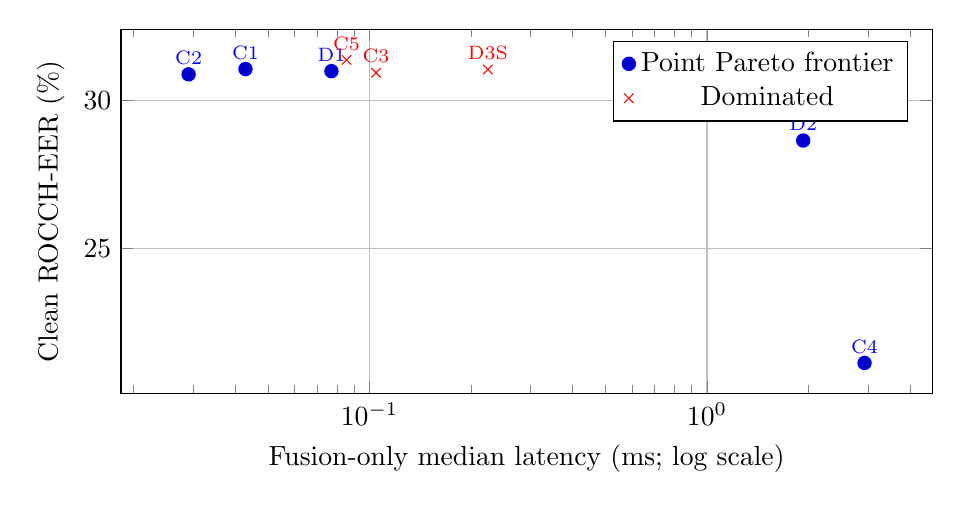
\begin{tikzpicture}
\begin{axis}[width=0.98\columnwidth,height=6.2cm,xmode=log,xlabel={Fusion-only median latency (ms; log scale)},ylabel={Clean ROCCH-EER (\%)},grid=major,legend pos=north east,point meta=explicit symbolic,nodes near coords,nodes near coords style={font=\scriptsize,anchor=south}]
\addplot+[only marks,mark=*,mark size=2.4pt] coordinates {(0.042879000,31.053879) [C1] (0.029089000,30.876043) [C2] (2.930127000,21.146749) [C4] (0.077098000,30.983505) [D1] (1.928308500,28.645278) [D2]};
\addlegendentry{Point Pareto frontier}
\addplot+[only marks,mark=x,mark size=2.4pt] coordinates {(0.104513500,30.928887) [C3] (0.085443500,31.362543) [C5] (0.224206000,31.040809) [D3S]};
\addlegendentry{Dominated}
\end{axis}
\end{tikzpicture}
\caption{Two visible Q2 dimensions. Pareto membership is computed from all four locked dimensions, including robustness loss and $C_{llr}$.}
\label{fig:v1-q2-pareto}
\end{figure}
